\begin{abstract}

The University of Chicago's Data Science Institute (DSI) works with 11th Hour Project grantees to support environmental and human rights work. In this paper, we describe a collaboration with the Occidental Arts \& Ecology Center (OAEC) on their Fuels-to-Flows program, which stabilizes upland waterways by adding brushwood that would otherwise fuel forest fires. Gullies are hidden by trees, so we used publicly available, sub-meter resolution LiDAR data to identify gullies by the shape of the landscape throughout Sonoma County, California. Due to the limited size of hand-labeled training datasets, we built an alternative to a Convolutional Neural Network (CNN) by engineering convolutional kernels using domain-specific knowledge---a ``right-sized machine learning'' solution for this problem---then identified gully centerlines and built a network of gullies as paths. The final deliverable is a statically hosted map application that puts all available information into the hands of restoration practitioners and land managers: the gully network, forest fire fuel proxies, aerial imagery, elevation contours, cross-sectional profiling tools, and differences in elevation between two LiDAR scans in 2013 and 2022. In this paper, we also describe how we overcame technological problems: CUDA programming in Python using Numba to handle our unusually large convolution kernels, PMTiles to serve hundreds of gigabytes of map data as a static website, and cross-sectional profiling tools.

\end{abstract}

\section{Introduction}

Through a partnership with the Schmidt Family Foundation's 11th Hour Project, the University of Chicago's Data Science Institute (DSI) contributes statistical and computational expertise to programs working for renewable energy, resilient food systems, healthy oceans, and the protection of human rights. The project described in this paper benefits the Occidental Arts \& Ecology Center (OAEC)'s Fuels-to-Flows program~\citep{Dolman2025FuelsToFlows}\citep{OAECGullyStuffing}, an innovative effort to solve two environmental problems, wildfires and erosion, in one stroke. Rather than eliminating brushwood that would fuel forest fires using controlled burns, this program packs that brushwood into small upland gullies to slow down runoff and retain water in the landscape.

We at the DSI were originally consulted to help find new sites for the Fuels-to-Flows program by scanning LiDAR data to find gullies and forest fire fuels in Sonoma County, California. Derived LiDAR products for forest fire fuels, ``ladder fuel proxies,'' were already provided by the SonomaVegMap project~\citep{SonomaVegMap} as publicly available data products, so we focused on identifying gullies.

Through our interactions with the OAEC, we learned that site selection for any environmental restoration work is a complex process that requires many considerations beyond listing the intersection of gullies with forest fire fuels. Land ownership, permitting constraints, accessibility, recent landscape change, and hazards invisible to LiDAR all contribute. Also, practitioners usually focus on a single park or wildlife reserve because of an ongoing relationship. Rather than providing a spreadsheet of candidate locations, it would be more effective to put the ability to explore the data in their hands, so we built a web-based map application that reveals all data pertinent to site selection: where the gullies are, where the forest fire fuels are, land ownership boundaries, aerial imagery corresponding to both full-county LiDAR sweeps in 2013 and 2022, elevation contours, differences in elevation between the two LiDAR sweeps, which is a proxy for erosion and deposition, and a tool for extracting detailed elevation cross-sections across landscape features from both years, which is useful for identifying migrating head-cuts, for instance. This map application doesn't replace the need to investigate sites in person, but it is invaluable for triaging and prioritizing sites.

Our goal for this paper is to provide a case study in how data science techniques and Python libraries were applied to solve a mission-driven problem in practice, highlighting the issues and pragmatic solutions, rather than presenting an idealized model of gully detection.

\section{Problem Context}

The Fuels-to-Flows program has been successfully applied on OAEC's own property and at Monte Rio Redwoods Regional Park over the last four years. The challenge now is to expand the program to new sites that the practitioners are not as intimately familiar with.

Most gullies are hard or impossible to find by aerial photography because they are hidden under a tree canopy, but they can easily be seen using bare-earth elevation maps derived from LiDAR scans. Airborne LiDAR instruments emit laser pulses and record reflected returns, some of which reflect from the tops of trees while others pass through gaps in the vegetation and reflect off the ground. The bare-earth elevation is derived from the ground returns and from interpolations through a 3-dimensional model of especially dense vegetation. The SonomaVegMap project published bare-earth elevation maps for the entire county with a 1~meter resolution in 2013 and a half-meter resolution in 2022.

Our geographic scope is the entirety of Sonoma County. The methods are not intrinsically limited to one county, but the available data products make the county a convenient boundary and it is already a significant expansion beyond the OAEC and its local collaborators. In addition, Sonoma County is somewhat unusual in having repeat coverage, which we can use to estimate landscape changes due to erosion. That said, the kernel length scales were chosen for the gully morphology visible in Sonoma County's half-meter bare-earth data, so regions with substantially different terrain or coarser, sparser LiDAR would likely require rescaling the kernels and re-fitting the model.

The main deliverable of this work is a web-based map in which all data layers can be overlaid for comparison. Some of those layers are directly copied from SonomaVegMap, such as ladder fuel proxies (e.g.\ LiDAR density 1--4~meters above ground divided by LiDAR density 0--4~meters above ground), or the Sonoma County GIS for parcel files for land ownership boundaries, with reformatting to provide them as map tiles. Other layers required significant derivation, such as the network of gullies that can be overlaid on other images. All of these data products are hosted on Cloudflare with documentation on our website, {\small \url{https://github.com/dsi-clinic/gully-map}}, to allow experts to dynamically load them in ArcGIS or QGIS. However, our web-based map is easier for non-experts and does not require extra software. Table~\ref{tab:data-products} summarizes all of the data products.

\begin{table}
\centering
\small
\begin{tabular}{l l l r}
\toprule
Layer & Derivation & Formats & Size \\
\midrule
Land ownership boundaries & Reformatted from Sonoma County GIS & PMTile & 27 MiB \\
Ladder fuel proxies & Reformatted from SVM 2022 & PMTile, GeoTIFF & 115 MiB \\
Greyscale hillshade & Reformatted from SVM 2022 & PMTile, GeoTIFF & 2.9 GiB \\
Color-enhanced hillshade & Derived from SVM 2022 data & PMTile, GeoTIFF & 149 GiB \\
Elevation contours & Derived from SVM 2022 data & PMTile, GeoJSON & 17.7 GiB \\
Elevation difference & Derived from SVM 2013 \& 2022 data & PMTile, GeoTIFF & 5.7 GiB \\
Elevation difference contours & Derived from SVM 2013 \& 2022 data & PMTile, GeoJSON & 11.8 GiB \\
Gully probability & Derived from SVM 2022 data & PMTile & 843 MiB \\
Detected gully network & Derived from SVM 2022 data & PMTile, Parquet & 34 MiB \\
Elevation 2013 \& 2022 & Reformatted from SVM 2013 \& 2022 & PMTile, GeoTIFF & 22.1 GiB \\
\bottomrule
\end{tabular}

\caption{Data products produced by this study, for viewing in the web-based map or directly in ArcGIS or QGIS. Here, ``SVM'' refers to SonomaVegMap and ``Size'' includes only PMTiles.\label{tab:data-products}}
\end{table}

\section{Gully Detection Model}

Two of the map features listed in Table~\ref{tab:data-products} are useful for finding gullies: color-enhanced hillshade, which is a raster image, and the detected gully network, which is vector data.

\subsection{Color-Enhanced Hillshade}

Color-enhanced hillshade, suggested by Adam Cummings, is derived from the bare-earth elevation map to make creases in the landscape more visible by eye. It consists of the elevation data $I_{\mathrm{in}}$, a function of spatial $x$ and $y$, texture-enhanced by a separable frequency-domain filter~\citep{textureshading},
\[ I_{\mathrm{out}} = \mathcal{F}^{-1}_x\!\left[(u^2)^\alpha \,\mathcal{F}_x(I_{\mathrm{in}})\right] +
\mathcal{F}^{-1}_y\!\left[(v^2)^\alpha \,\mathcal{F}_y(I_{\mathrm{in}})\right] \]
where $\mathcal{F}_x$ and $\mathcal{F}_y$ are horizontal and vertical Fourier transformations, $u$ and $v$ are the corresponding frequency coordinates, and $\alpha = 0.5$. The resulting image $I_{\mathrm{out}}$ is then mapped to a blue-green-yellow color ramp and combined with a grayscale hillshade (derived from the same elevation data $I_{\mathrm{in}}$) using the overlay blend mode:
\[
\text{overlay}(x, y) = \left\{\begin{array}{c l}
2 x y & \textrm{if } y < 0.5 \\
1 - 2 (1 - x) (1 - y) & \textrm{otherwise.}
\end{array}\right\}
\]
This effectively colorizes the hillshade with the texture-enhanced relief signal. A sample of this transformation is shown in the top half of Figure~\ref{fig:banner}.

\begin{figure}
\centering

\includegraphics[width=\textwidth]{img/banner.png}
\caption{Sample imagery in which the top two panels are color-enhanced hillshade and the bottom two panels are aerial photography from 2022. In the middle two panels, the detected gully network is drawn as outlined blue paths.\label{fig:banner}}
\end{figure}

\subsection{Detected Gully Network}

Although the color-enhanced hillshade draws the eye's attention to subtle creases, it can't be overlaid on other image layers such as a street map or aerial photography, which are sometimes needed for surrounding context. For a clean overlay, we want a vectorized path that can be outlined without introducing too much visual noise.

To produce such a path, we first need to identify which pixels in the bare-earth elevation image are in gullies, then connect neighboring gully pixels to form a graph whose nodes are the pixels, and finally skeletonize the graph to narrow it to uniform (single pixel) thickness.

The first step, identifying pixels in gullies, affects the final quality of the network. If too many pixels are identified, the final network will be noisy, with many disconnected short paths. If too few pixels are identified, gullies will be missed. In a standard technique, called Difference From Mean Elevation (DFME) and described for instance by Evans and Lindsay~\citep{evans2010}, the elevation at each pixel is subtracted from the mean elevation in a large square or circle centered on that pixel. It is often used directly as an imaging technique, like color-enhanced hillshade. To use this algorithm as a first step in graph-building and skeletonization, we need to set a threshold to label deep indentations as gullies, but there is no threshold that accepts enough pixels without also accepting too much noise. The landscape has many dimples that are as deep as a gully without being connected to a system of channels like a gully.

At the other extreme, we could use a Convolutional Neural Network (CNN) to identify gullies as an image segmentation problem. However, this supervised learning technique requires a target dataset of pixels that have already been labeled as ``gully'' or ``not gully.'' Since we had no such dataset, we hand-labeled training data on our own by painting over images with one color for ``gully,'' another for ``not gully,'' and transparency wherever a determination could not be made. This was a time-consuming process involving ground-truth checking with Google Street View, separately in 9~watersheds of Sonoma County for geographic variety. In the end, we did not have enough hand-labeled data to train a CNN.

There is a midpoint between these extremes. The DFME method is a convolution of the image with a kernel that is positive at a central point, negative in a large square or circle centered on that point, and sums to zero:
\[
K_{\mathrm{DFME}}(x,y)=
\left\{\begin{array}{c l}
\dfrac{1}{\pi w^2} & \textrm{if } x^2+y^2\le w^2 \\
-\dfrac{1}{\pi(R^2-w^2)} & \textrm{if } w^2<x^2+y^2\le R^2 \\
0 & \textrm{otherwise}
\end{array}\right\}
\]
for $w$ = 1 pixel and $R$ = 50 pixels (25~meters), illustrated on the left of Figure~\ref{fig:kernels}. Convolving this kernel with the bare-earth elevation image effectively subtracts each pixel from the mean of all pixels in a circle of radius $R$ around it.

A convolutional layer in a CNN convolves the image with several kernels that are learned as part of the global optimization. The kernels represent relevant shapes at different size scales by pooling (resizing) the image in each layer. While that's necessary for recognizing complex images like the face of a cat with sufficient generality to be insensitive to camera angles and lighting, our task is much simpler: gullies are trough-shaped and the Earth is always viewed from directly above. Instead of convolving with $K_{\mathrm{DFME}}$, we can convolve with a trough-shaped kernel,
\[
K_{\mathrm{trough}}(x,y;\theta, \sigma)=
\left\{\begin{array}{c l}
-1/(\pi R^2)
+\dfrac{\exp\!\left(-\dfrac{x^2+y^2}{2\sigma^2}\right)}
{\text{normalization}}
& \text{if } x^2+y^2\le R^2 \text{ and } |x\sin\theta+y\cos\theta|<w \\
-1/(\pi R^2)
& \text{if } x^2+y^2\le R^2 \text{ and } |x\sin\theta+y\cos\theta|\ge w \\
0
& \text{otherwise}
\end{array}\right\}
\]
where $K_{\mathrm{trough}}$ is parameterized by an angle $\theta$, illustrated in the middle of Figure~\ref{fig:kernels}. A convolution with this kernel highlights pixels that are lower than the surrounding region and also part of a linear path of low pixels, a path angled by $\theta$ and tapered like a Gaussian with characteristic length $\sigma$. Performing a weighted sum over such kernels at a variety of angles $\theta$ highlights pixels in troughs of any direction, and this process is equivalent to inference in one convolution layer of a CNN.

In practice, we noticed that convolutions with $K_{\mathrm{trough}}$ also highlighted one-sided cliffs, usually artificial cliffs along roadsides, because the cliff matches one side of a trough and missing the other side only dampens the convolution by a factor of 2. As a veto, we added another kernel that only matches one-sided cliffs:
\[
K_{\mathrm{cliff}}(x,y;\theta, \sigma)=
\left\{\begin{array}{c l}
\dfrac{1}{\text{normalization}} \, {\exp\!\left(-\dfrac{x^2+y^2}{2\sigma^2}\right)}
& \text{if } x^2+y^2\le R^2 \text{ and } x\sin\theta+y\cos\theta < 0 \\
-\dfrac{1}{\text{normalization}} \, {\exp\!\left(-\dfrac{x^2+y^2}{2\sigma^2}\right)}
& \text{if } x^2+y^2\le R^2 \text{ and } x\sin\theta+y\cos\theta \ge 0 \\
 \, 0
& \text{otherwise,}
\end{array}\right\}
\]
illustrated on the right of Figure~\ref{fig:kernels}. A model that gives positive weight to convolutions with $K_{\mathrm{trough}}$ and negative weight to convolutions with $K_{\mathrm{cliff}}$ can distinguish between troughs and cliffs.

\begin{figure}
\centering
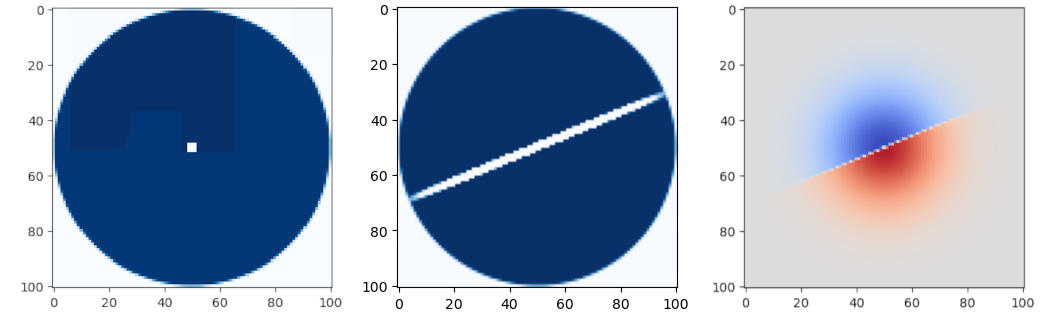
\includegraphics[width=\textwidth]{img/kernels.png}

\caption{Convolution kernels for pixelwise gully detection. Left: the DFME kernel ($K_{\mathrm{DFME}}$) is positive in one pixel in the center, negative in a large disk around it, and sums to zero. Middle: a trough-shaped kernel ($K_{\mathrm{trough}}$) replaces the single positive pixel with an angled line of a characteristic length $\sigma$, tapered as $\exp(-x^2/\sigma^2)$. Right: the cliff veto kernel ($K_{\mathrm{cliff}}$) is a positive (red) Gaussian on one side of an angled line and negative (blue) on the other.\label{fig:kernels}}
\end{figure}

To be clear, we are replacing a learned-kernel CNN with feature engineering inspired by CNNs. We are using domain knowledge to hand-craft a set of kernels. We also know that convolutions with $K_{\mathrm{trough}}(x,y;\theta, \sigma)$ should have a roughly sinusoidal dependence on $\theta$ for a point in a linear gully with a stronger dependence if $\sigma$ is large because the kernel shape is a good fit when aligned and a bad fit when misaligned. We verified this for several points in gullies, one of which is shown in Figure~\ref{fig:connected-gullies-single-pixel}.

\begin{figure}
\centering
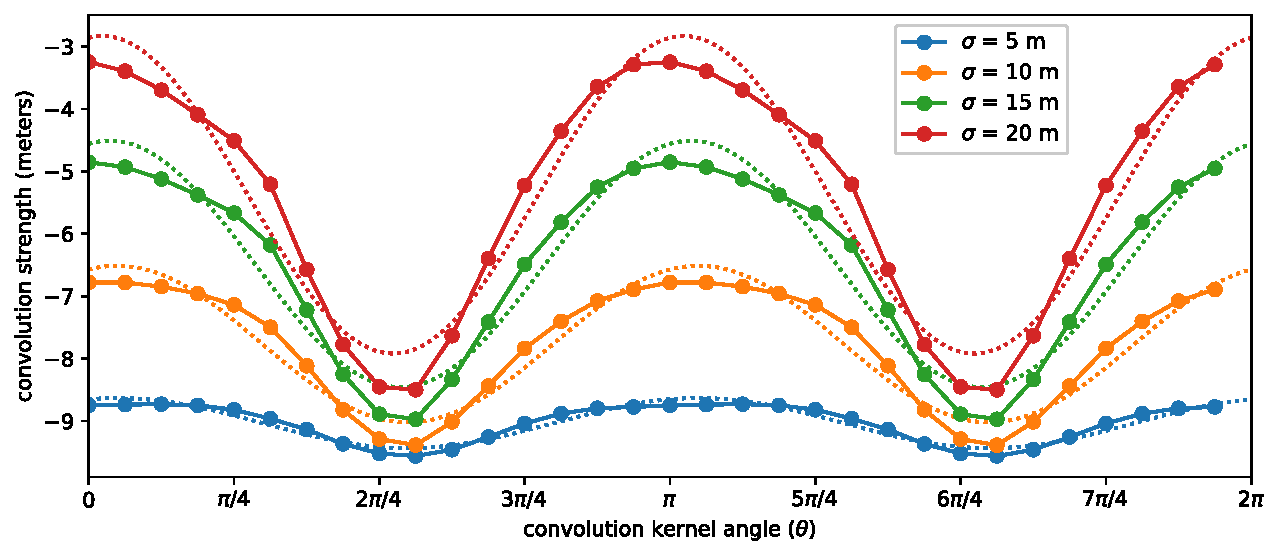
\includegraphics[width=0.8\textwidth]{img/connected-gullies-single-pixel.pdf}

\caption{Value of convolutions at a point in a gully for $K_{\mathrm{trough}}(x,y;\theta)$ with varying angles $\theta$ and Gaussian widths $\sigma$. Dotted lines are sinusoidal fits to the convolution results. \label{fig:connected-gullies-single-pixel}}
\end{figure}

Due to this regularity, we can reduce the number of features and therefore the number of parameters in the model without losing model
quality. The three most important features are the highest and lowest point of a sinusoidal fit of convolutions $C(x, y; \theta, \sigma)$ with kernel $K_{\mathrm{trough}}(x,y;\theta, \sigma)$ and the minimum value of those convolutions, which is useful because the minimum value is lower than the fitted sinusoidal curve in most of the real gullies that we observed. The amplitude of the sinusoidal fit can be computed directly as the modulus of a complex sum, a Riemann approximation of the integral to compute the first Fourier coefficient. The phase of the sinusoidal fit could tell us the direction of the trough at a given point, but we don't need that for modeling.
\[
  \textrm{high}(x, y; \sigma) = \frac{1}{16}\sum_{n=0}^{15} C(x, y; {\frac{n}{16}\pi}, \sigma) + \frac{1}{8}\left| \sum_{n=0}^{15} C(x, y; {\frac{n}{16}\pi}, \sigma) e^{i n\pi/8} \right|
\]
\[
  \textrm{low}(x, y; \sigma) = \frac{1}{16}\sum_{n=0}^{15} C(x, y; {\frac{n}{16}\pi}, \sigma) - \frac{1}{8}\left| \sum_{n=0}^{15} C(x, y; {\frac{n}{16}\pi}, \sigma) e^{i n\pi/8} \right|
\]
\[
  \textrm{mini}(x, y; \sigma) = \min_{n=0}^{15} \, C(x, y; {\frac{n}{16}\pi}, \sigma).
\]
To exclude cliffs, we take the minimum of convolutions $C_{\textrm{cliff}}(x, y; \theta, \sigma)$ with kernel $K_{\mathrm{cliff}}(x, y; \theta, \sigma)$.
\[
  \textrm{cliff}(x, y; \sigma) = \min_{n=0}^{15} \, C_{\textrm{cliff}}(x, y; {\frac{n}{16}\pi}, \sigma). \\
\]
Evaluating these at $\sigma$ = 5~meters and 15~meters,
\[
\begin{array}{l l}
H_5(x, y) = \textrm{high}(x, y; \textrm{5~meters}) & H_{15}(x, y) = \textrm{high}(x, y; \textrm{15~meters}) \\
L_5(x, y) = \textrm{low}(x, y; \textrm{5~meters}) & L_{15}(x, y) = \textrm{low}(x, y; \textrm{15~meters}) \\
M_5(x, y) = \textrm{mini}(x, y; \textrm{5~meters}) & M_{15}(x, y) = \textrm{mini}(x, y; \textrm{15~meters}) \\
& F_{15}(x, y) = \textrm{cliff}(x, y; \textrm{15~meters}) \\
\end{array}
\]
we performed a logistic regression with parameters $a_i$ and bias term $b$
\begin{equation}\label{eqn:logistic-fit}
\begin{aligned}
\textrm{logit}(p) =& \text{ }a_1 M_{15} + a_2 (L_{15} - M_{15}) + a_3 (H_{15} - L_{15}) + a_4 (M_5 - M_{15}) \\
&+ a_5 (H_5 - L_5) + a_6 L_{15}(H_{15} - L_{15}) + a_7 \left| F_{15} \right| + b
\end{aligned}
\end{equation}
over all pixels $x$, $y$ and obtained the results shown in Table~\ref{tab:fit-results}. The fitted model's predicted probabilities for pixels labeled as ``not in gully'' or ``in gully'' are shown for the 9~watersheds in Figure~\ref{fig:residuals}; note that these are in-sample residuals. The dominant term is $M_{15}$, the minimum convolution with $\sigma = 15$~meter troughs. Because $M_{15}$ values are negative in gullies with a negative coefficient, this term contributes positively to the probability that a pixel is in a gully. The rest of the terms are amplitudes, one interaction term, and the cliff veto. The cliff veto is fitted in absolute magnitude because it has an antisymmetry for $\theta \to \theta + \pi$. Because it is always positive and has a negative coefficient, it contributes negatively to the probability that a pixel is in a gully. Figure~\ref{fig:cross-validation} provides an out-of-sample measure of model quality: the Area Under the Curve (AUC) of the Receiver Operating Characteristic (ROC), cross-validated across the 9~watersheds. All AUC values are above 0.98, indicating not only good discriminating power, but also consistency across watersheds.

\begin{figure}
\centering
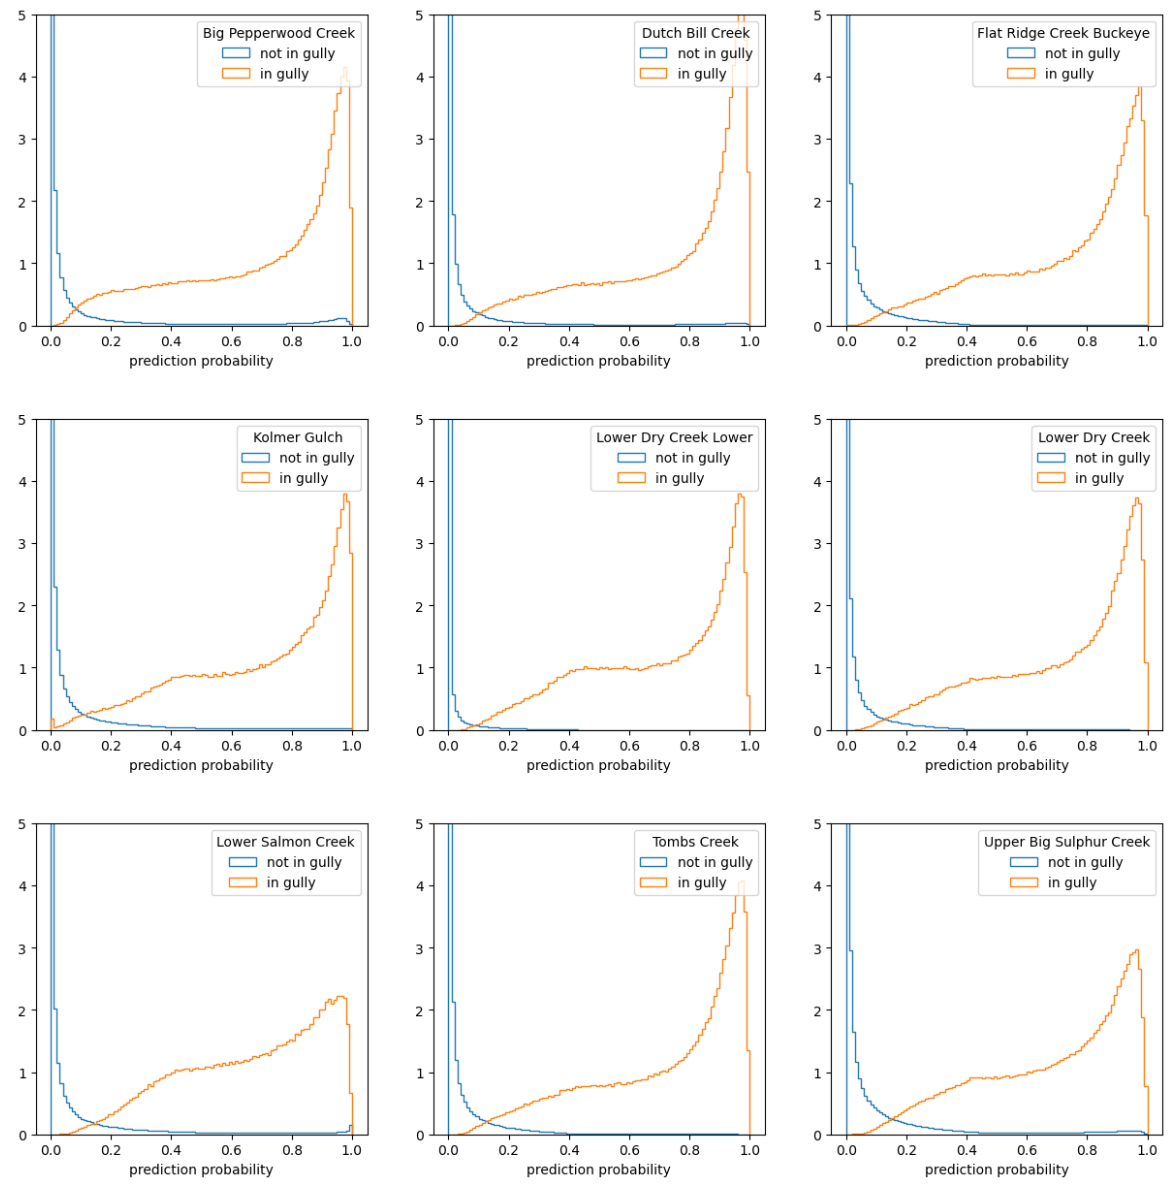
\includegraphics[width=\textwidth]{img/residuals.png}

\caption{Predicted probability for pixels labeled as ``not in gully'' or ``in gully'' in 9~watersheds. These pixels were used to train the 8~parameter fit, so they are in-sample residuals (difference of ``not in gully'' from 0 and difference of ``in gully'' from 1).\label{fig:residuals}}
\end{figure}

\begin{figure}
\centering
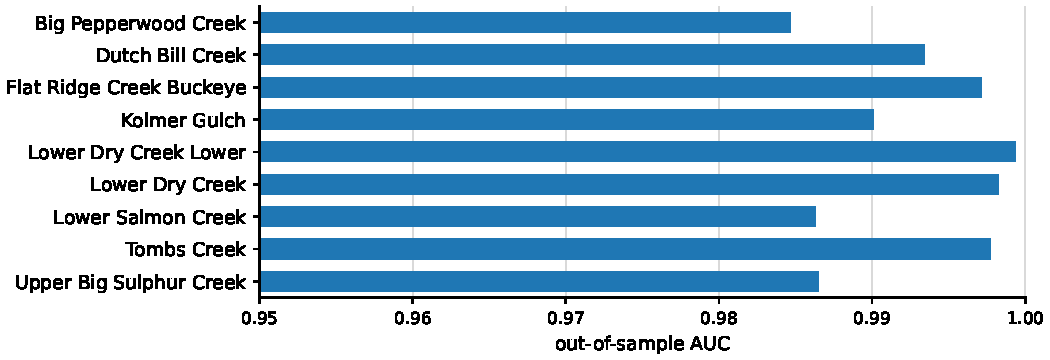
\includegraphics[width=\textwidth]{img/cross-validation.pdf}

\caption{Area Under the Curve (AUC) of the Receiver Operating Characteristic (ROC) for gully-finding models cross-validated across the 9~watersheds.\label{fig:cross-validation}}
\end{figure}

\begin{table}
\centering
\small
\begin{tabular}{c c c | c c c}
\toprule
parameter & value & term & parameter & value & term \\
\midrule
$a_1$ & $\,-3.16$ & $M_{15}$ & $a_5$ & $\,-0.27$ & $(H_5 - L_5)$ \\
$a_2$ & $\,-0.72$ & $(L_{15} - M_{15})$ & $a_6$ & $\,\,\,0.63$ & $L_{15}(H_{15} - L_{15})$ \\
$a_3$ & $\,\,\,1.94$ & $(H_{15} - L_{15})$ & $a_7$ & $\,-0.29$ & $\left| F_{15} \right|$ (cliff veto) \\
$a_4$ & $\,\,\,0.20$ & $(M_5 - M_{15})$ & $b$   & $\,-9.80$ & (bias/intercept) \\
\bottomrule
\end{tabular}

\caption{Fit results for the logistic regression in Equation~\ref{eqn:logistic-fit}.\label{tab:fit-results}}
\end{table}

Since the terms of the logistic regression are not all linear combinations of the convolutions, our model has diverged from a standard CNN, but it's still advantageous to add a second ``layer'' to clean the image further. This subsequent step consisted in shrinking the image by a factor of 2 (pooling) and convolving again, this time with $K_{\mathrm{trough}}(x,y;\theta, \sigma)$ with $\sigma = 20$~meters and minimize over 16 grid-points in $\theta$. Figure~\ref{fig:gully-finding-quality} illustrates the result for one gully system: (a)~shows the color-enhanced hillshade for reference, (b)~is the DFME method, (c)~shows a threshold applied to the DFME image to make a mask, then each connected component is shown in a different color, (d)~shows the probability output of this two-layer method, and (e)~is a similar mask colored by connected components with a probability $>$ 5\% threshold. Compared with DFME, the two layers of trough convolutions produce a considerably less noisy image with the main gully's connections intact.

\begin{figure}
\centering
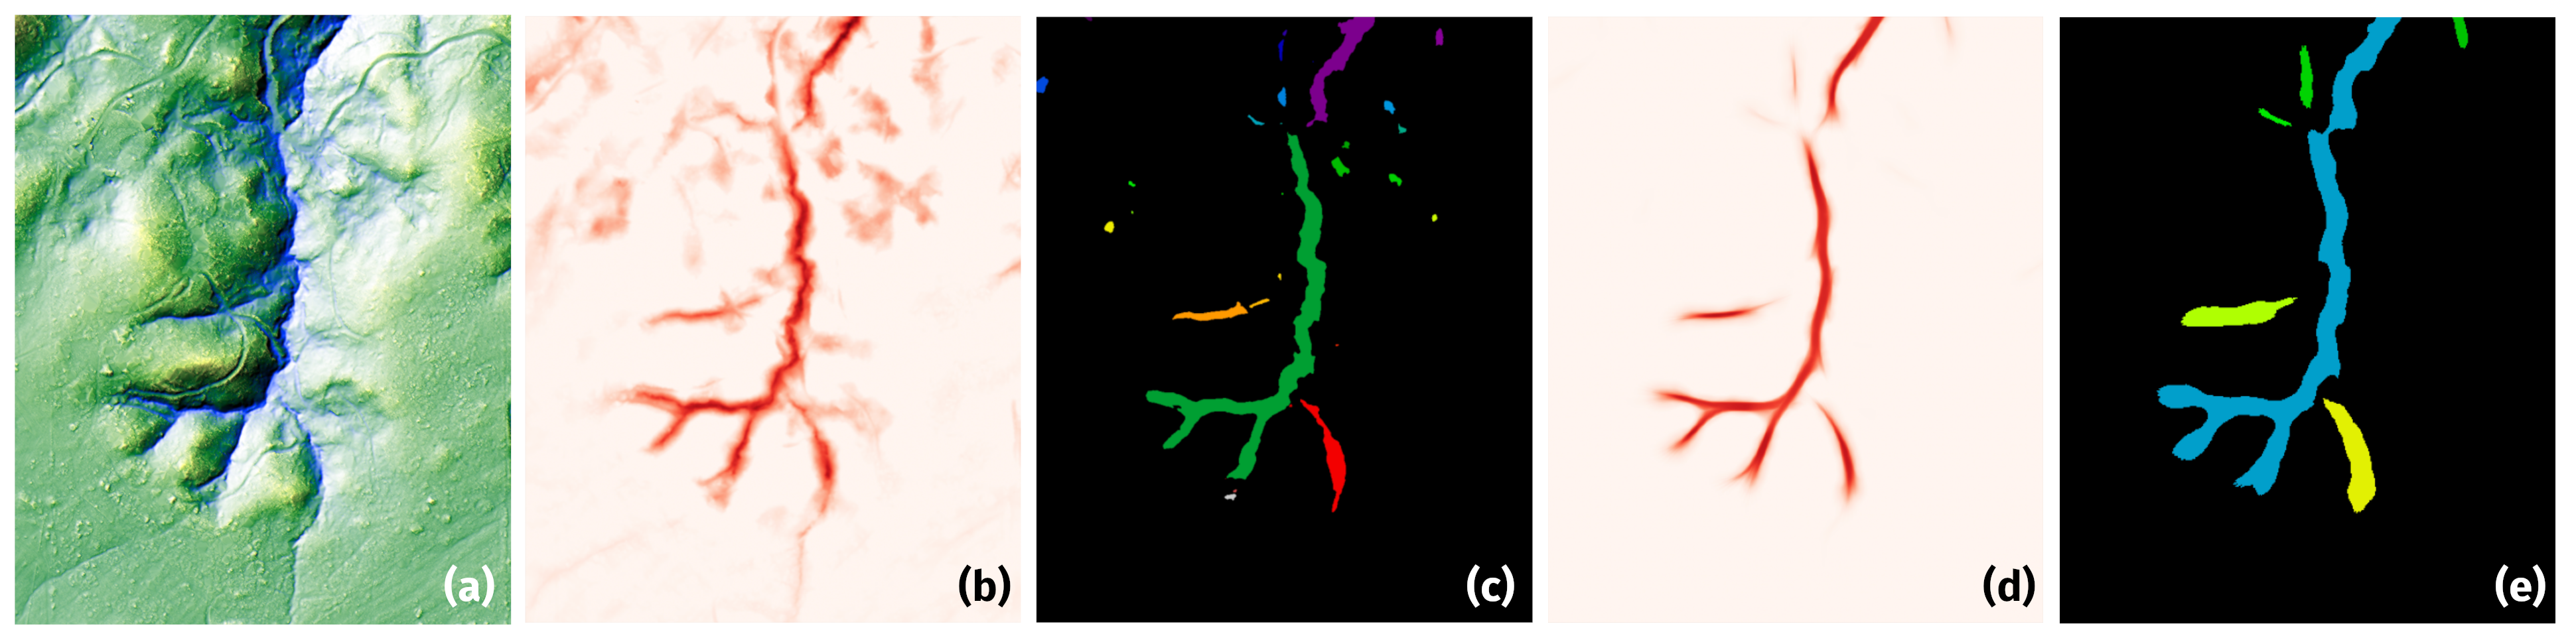
\includegraphics[width=\textwidth]{img/gully-finding-quality.png}

\caption{Comparison of gully-finding algorithms: (a)~color-enhanced hillshade, (b)~DFME, \\ (c)~its connected components, (d)~two-layer trough convolution, (e)~its connected components.\label{fig:gully-finding-quality}}
\end{figure}

The next step is to reinterpret the above-threshold pixels of the image as nodes in a graph, connected with any neighbors on their 8~sides, and skeletonize the image by removing nodes if removing them does not change the connectivity of the graph. We implemented a greedy algorithm that removes pixels in increasing order of probability, so that the threshold could be set very low: probability $>$ 1\%. To see why such a low threshold is needed, see Figure~\ref{fig:residuals}: distributions of non-gully probability peaks near 0, but gully pixels, which are much less numerous in the data, are more uniform from 0 to 1. The skeletonization and its resulting graph are shown in Figure~\ref{fig:skeletonization-and-graph-building}.

\begin{figure}
\centering
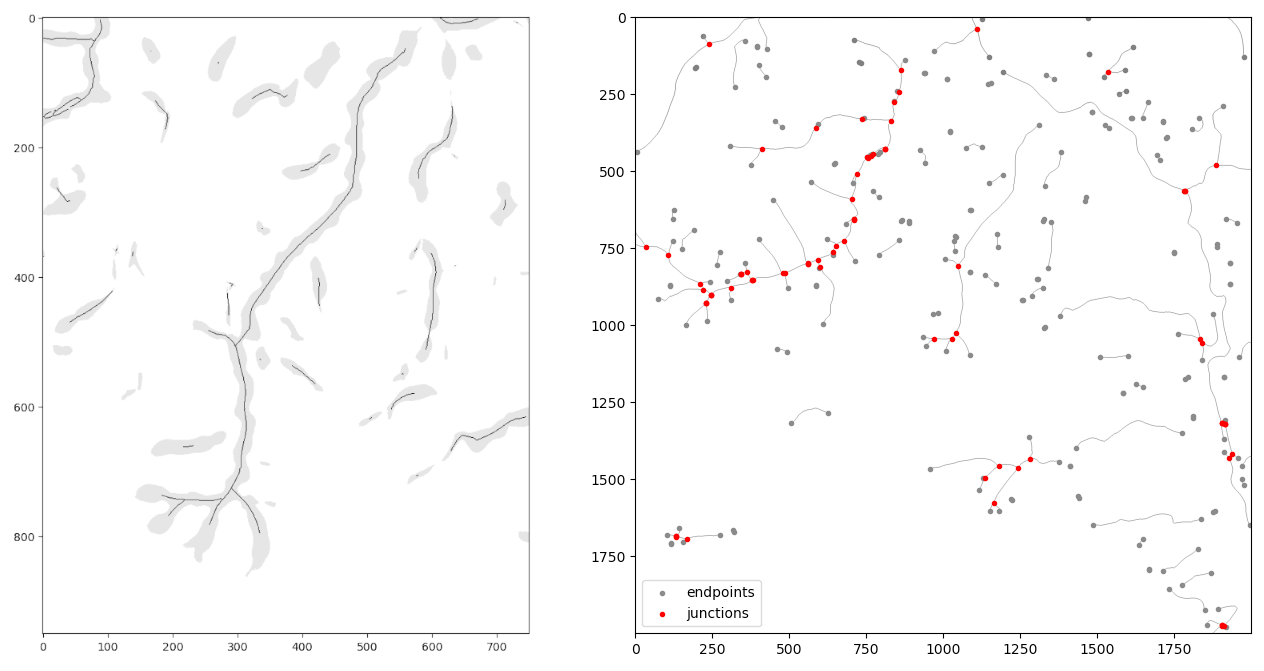
\includegraphics[width=\textwidth]{img/skeletonization-and-graph-building.png}

\caption{Left: skeletonization of 1\% probability threshold masks (gray) with probability-ordered erosion. Right: connection of the remaining pixels as a graph by identifying neighbors.\label{fig:skeletonization-and-graph-building}}
\end{figure}

\section{Performance Optimization with Numba}\label{sec:numba}

Some steps in the gully-finding analysis are similar to standard techniques, but with unusual scaling. Early in the analysis, we found that our convolution kernels needed to be at least 50~meters on a side to average over enough surrounding elevation for a stable baseline. Image convolution kernels are typically $3\times 3$ through $11\times 11$ pixels, but ours are $101\times 101$. The time spent computing convolutions with SciPy's \texttt{convolve2d} was a constraint on exploratory studies, so we searched for alternatives. First we considered \texttt{*.scipy.signal.convolve2d} drop-in GPU-based replacements from the CuPy~\citep{cupy} and JAX~\citep{jax} libraries, but the fastest implementation by a factor of several was a custom CUDA kernel compiled by Numba~\citep{numba} with a fixed kernel size at compile time and simplified boundary conditions. To eliminate sensitivity to boundary conditions, we performed each convolution on one watershed at a time with padded boundaries, then clipped to the watershed. Gullies cannot cross a watershed divide.

We also used a custom CUDA kernel compiled by Numba for skeletonization, since the methods in Scikit-Image apply to bitmaps with the probability information removed. We implemented a skeletonization algorithm similar to Pudney's distance-ordered homotopic thinning~\citep{PUDNEY1998404}, but we eroded pixels greedily in order of increasing probability, rather than distance, and we used connectivity-preservation as a constraint instead of topology-preservation, ensuring that all gullies are trees.

In both cases, we developed the analysis using standard libraries, then replaced the functions that needed better performance or different behavior with a CUDA kernel of the same API.

\section{Delivery as a Static Map Application}

Although the data products described in Table~\ref{tab:data-products} are accessible to geospatial applications like ArcGIS and QGIS, most of the intended consumers are not geospatial experts, so we built a web-based map application. This application has a conventional interface: a large scrollable map with switches in a sidebar to toggle layers.

Often, these map applications are built with a server to provide map tiles on demand. A custom server would require occasional maintenance, which scales poorly because the DSI develops applications for many projects, and servers must be maintained indefinitely. Maintenance could be offloaded to a service like MapTiler, but accumulating services with monthly fees is a different kind of maintenance scaling. The best option is to provide an application as a static website---files served by Cloudflare without any application logic outside of the user's web browser.

The map and sidebar are all client-side HTML built with Svelte. The data products add up to hundreds of GiB, which is far too much to load with the webpage; it will need to be dynamically loaded as tiles. A directory structure of XYZ tiles adds significant overhead and MBTiles require an active server to look up entries in an SQLite database. Instead, we used PMTiles~\citep{pmtiles}, a file format in which tiles are embedded at known seek positions within the file. A client-side library uses an index to find those seek positions, and then does a partial HTTP GET to access one tile at a time. All of the raster and vector data products are served as PMTiles.

The map application also allows users to draw a straight or curved line on the map for a cross-section of the elevation along that line, as shown in Figure~\ref{fig:dashboard}. The elevation data used for this calculation is also provided as PMTiles. Each 32-bit floating point number is cast as the RGBA channels of a PNG raster in PMTiles and then decoded on the client.

\begin{figure}
\centering
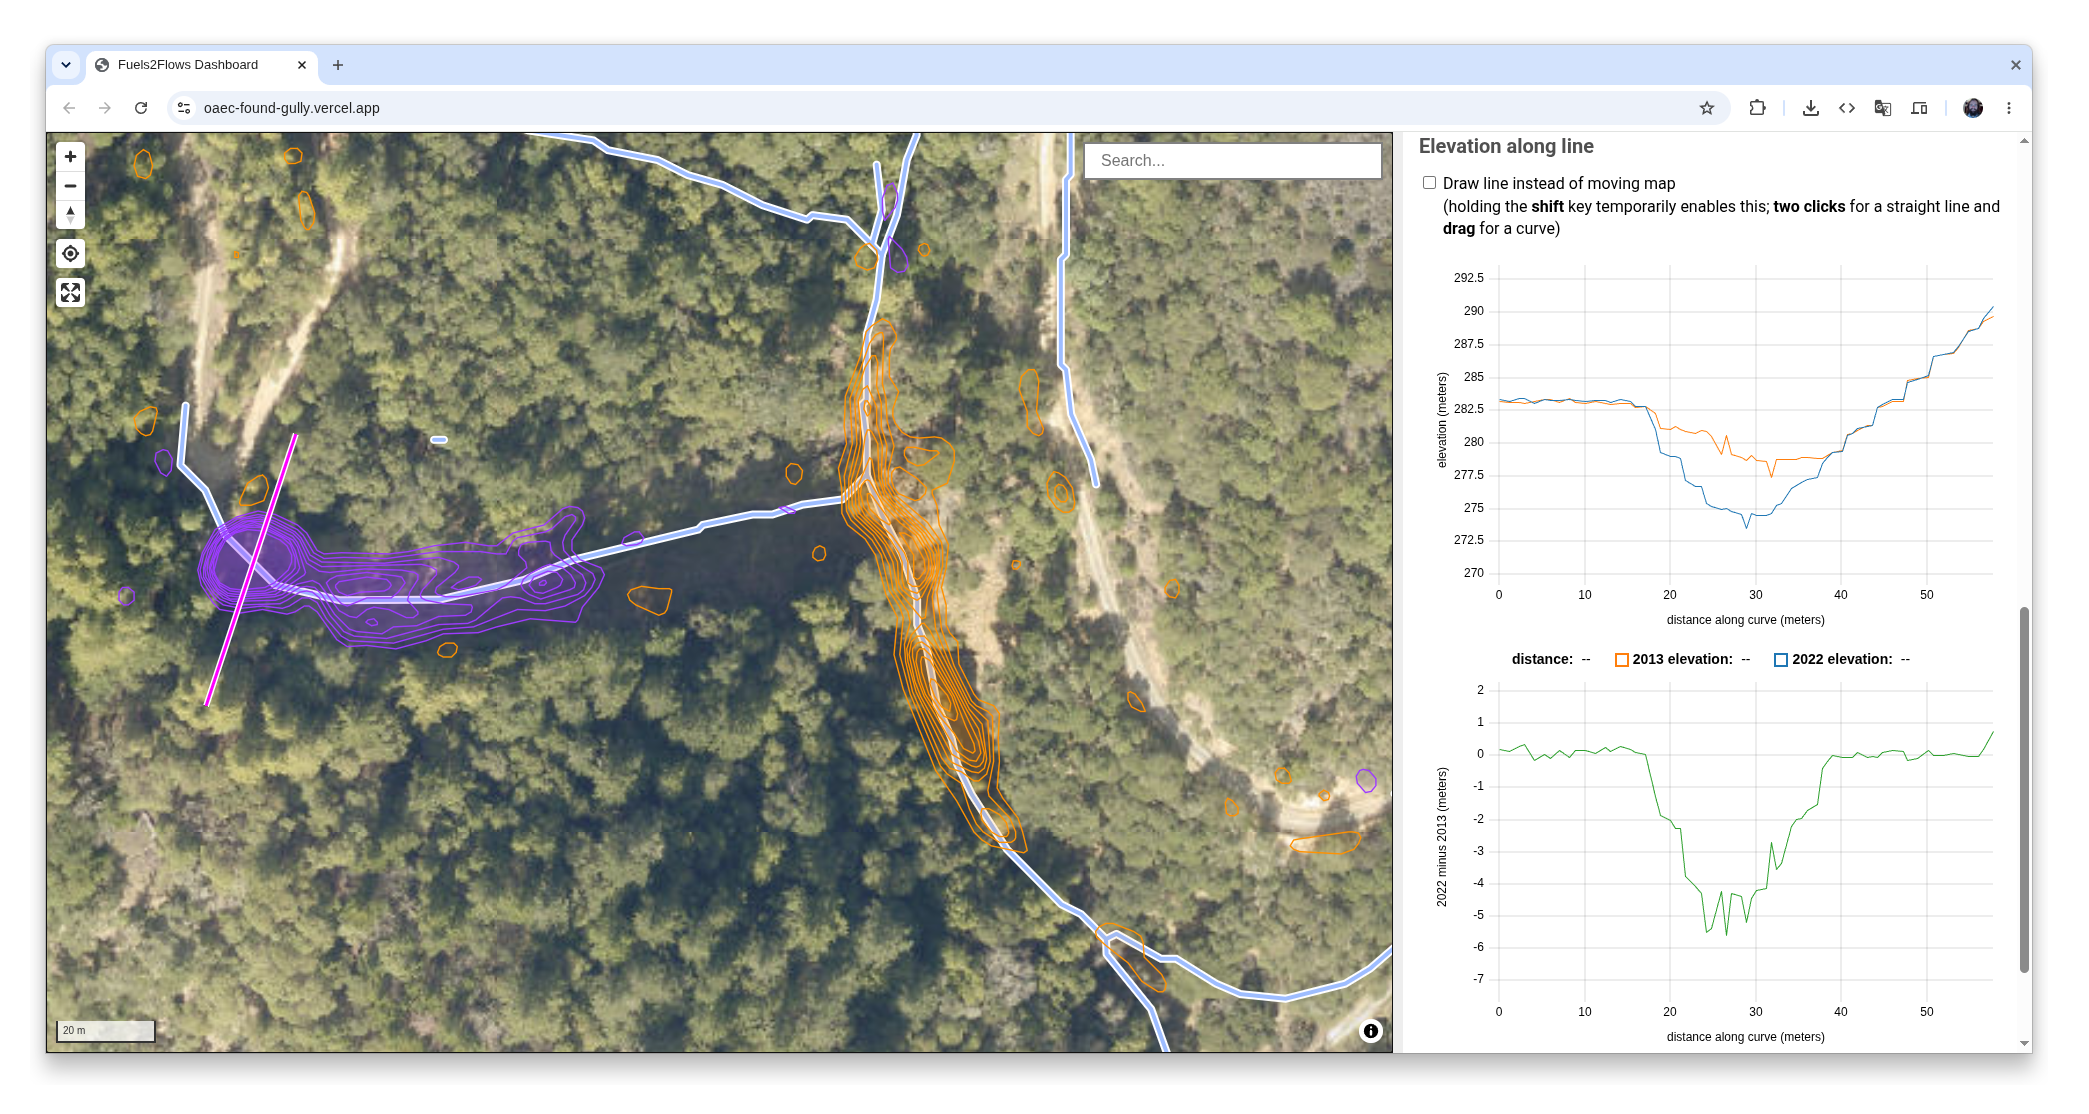
\includegraphics[width=\textwidth]{img/dashboard.png}

\caption{The web-based map application, showing 2021 aerial photography, gully paths (outlined light blue), erosion (purple) and deposition (orange) contours, and a user-drawn line (magenta) along which elevation in 2013, 2022, and their difference are displayed as plots on the right.\label{fig:dashboard}}
\end{figure}

The GitHub repository for this project is {\small \url{https://github.com/dsi-clinic/gully-map}}
where you will find a link to the map application, documented links to data products that can be loaded in ArcGIS or QGIS, and all of the code that was used to build it.

\section{Cross-Disciplinary Reach}

While the gully-finding study was underway, one of us was co-mentoring a University of Chicago Data Science Clinic project on an unrelated topic: a team of students were predicting pathologic complete response to treatment in breast cancer from MRI images using graph neural networks of the blood vessels. Building a graph from voxels identified as being in blood vessels is very similar to building a graph from pixels identified as being in blood vessels, except that MRI voxels are 3-dimensional while the LiDAR elevation map is 2-dimensional. Both studies need the connectivity achieved by setting segmentation thresholds low, and therefore they both benefit from the probability-ordered skeletonization algorithm described in Section~\ref{sec:numba}.

One of the students, Jos\'e Cardona, adapted the 2-dimensional skeletonization algorithm to 3-dimensional blood vessels and observed performance gains in the final analysis compared to using the Vascular Modeling Toolkit (VMTK) skeletonization module in 3D Slicer. In the following quarter, the algorithm was further generalized to 4-dimensional time-series of MRI images, and our co-mentor Anna Woodard is now applying it to high time-resolution imaging sequences beyond the scope of the Clinic course. This instance of cross-disciplinary transfer illustrates the value of generalist organizations like the DSI, as well as a tight relationship between research and teaching.

\section{Conclusions}

This project addressed a set of questions that are broadly relevant to the SciPy community, beyond the specifics of gully detection. In each case, the useful path was a middle ground between a fully general solution and a special-purpose one built from scratch.

\textbf{How can one build a model for inference on big datasets when training data are scarce?} We built a model \textit{inspired by} a CNN, but constructed it with domain-specific knowledge rather than a fully automated training process. This let us capture most of the benefit of a CNN's inductive bias without the quantity of supervision target data that optimizing convolution kernels would typically need. This relied on recognizing that the standard DFME technique is itself a convolution, thereby identifying a continuity between the two approaches from which we could choose a middle ground.

\textbf{What can one do if a computational technique breaks scaling assumptions or differs slightly from algorithms built into scientific libraries?} In a workflow that uses standard scientific Python libraries wherever possible, we replaced only the specific functions that didn't scale or differed from the standard algorithms. Numba allowed us to compile our alternative code for speed yet interface with standard NumPy and CuPy arrays so that the majority of the workflow would be untouched.

\textbf{How can one deliver large geoscience data products to users with varied technical expertise?} A custom web application is a user-friendly way to browse data, although map applications typically require active servers to deliver data one tile at a time, and active servers are a maintenance burden. Static websites with pinned JavaScript dependencies require comparatively little upkeep, and the PMTiles format can be addressed one tile at a time by client-side libraries.

We hope this case study is useful to others facing similar issues.

\section*{Acknowledgments}

We are grateful for Brock Dolman's very helpful guidance and useful feedback from Adam Cummings, Matt O'Connor, and Jeremy Kobor.
